%!TeX root = Chapter_Appendix
\documentclass[../../CompleteThesis/Complete_1stDraft.tex]{subfiles}
\begin{document}
\section[Appendix I]{Firn Diffusivity}
\label{App:FirnDiffusivity}


\section[Appendix II]{Data: AWI B-cores}
\label{App:Data_AWI}


\newpage
\begin{rotatepage}
	\begin{landscape}
		\begin{table}
			\centering
			\begin{tabular}{c||c||c}
				\textcolor{BrickRed}{\textbf{TERRIBLE}} & \textcolor{YellowOrange}{\textbf{REASONABLE}} & \textcolor{OliveGreen}{\textbf{GOOD}} \\
				\hline
				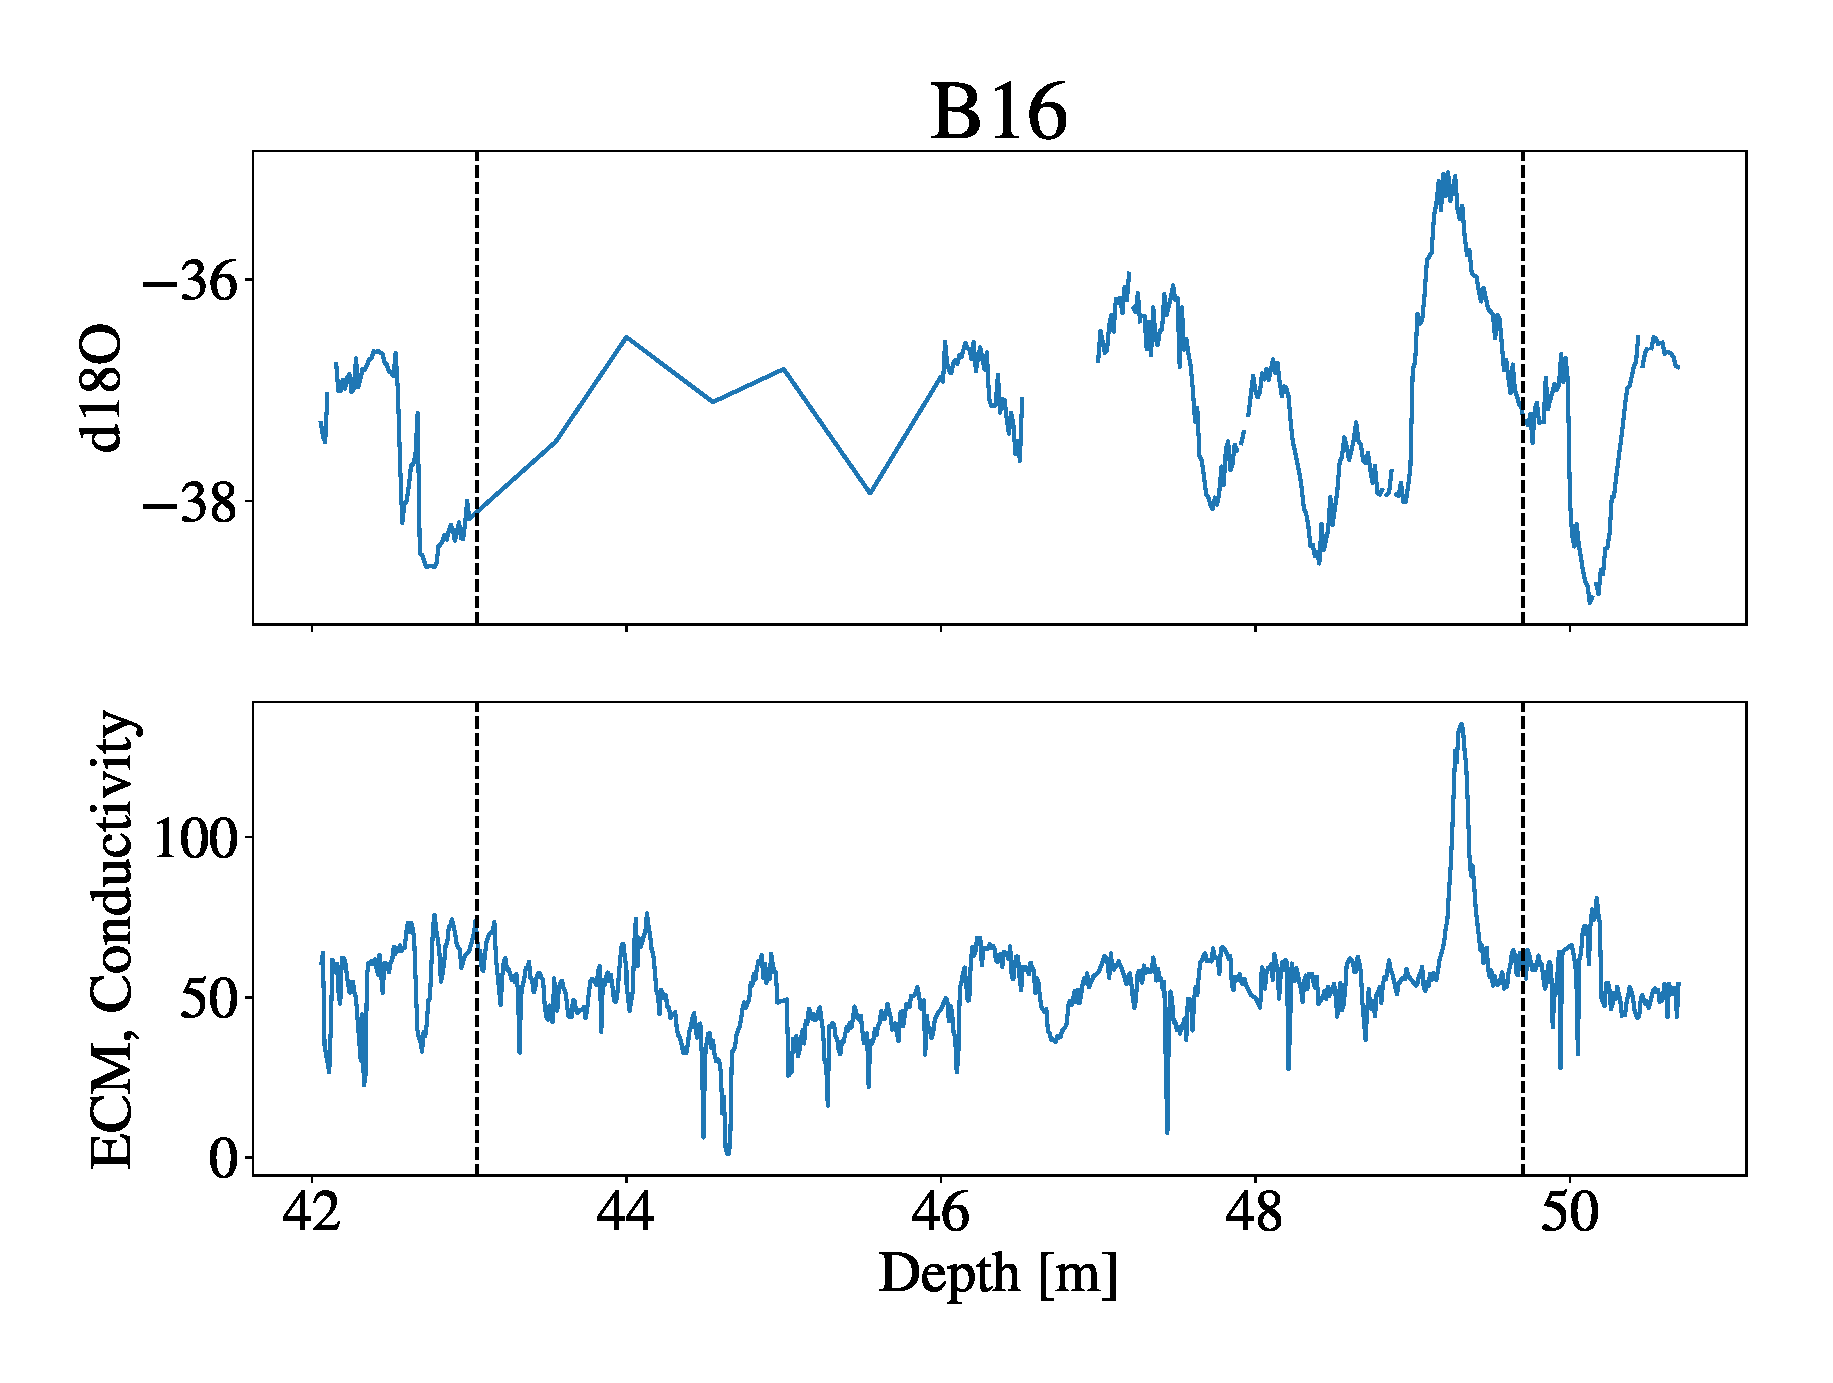
\includegraphics[width =0.3\linewidth]{Core_LT_B16.eps} & 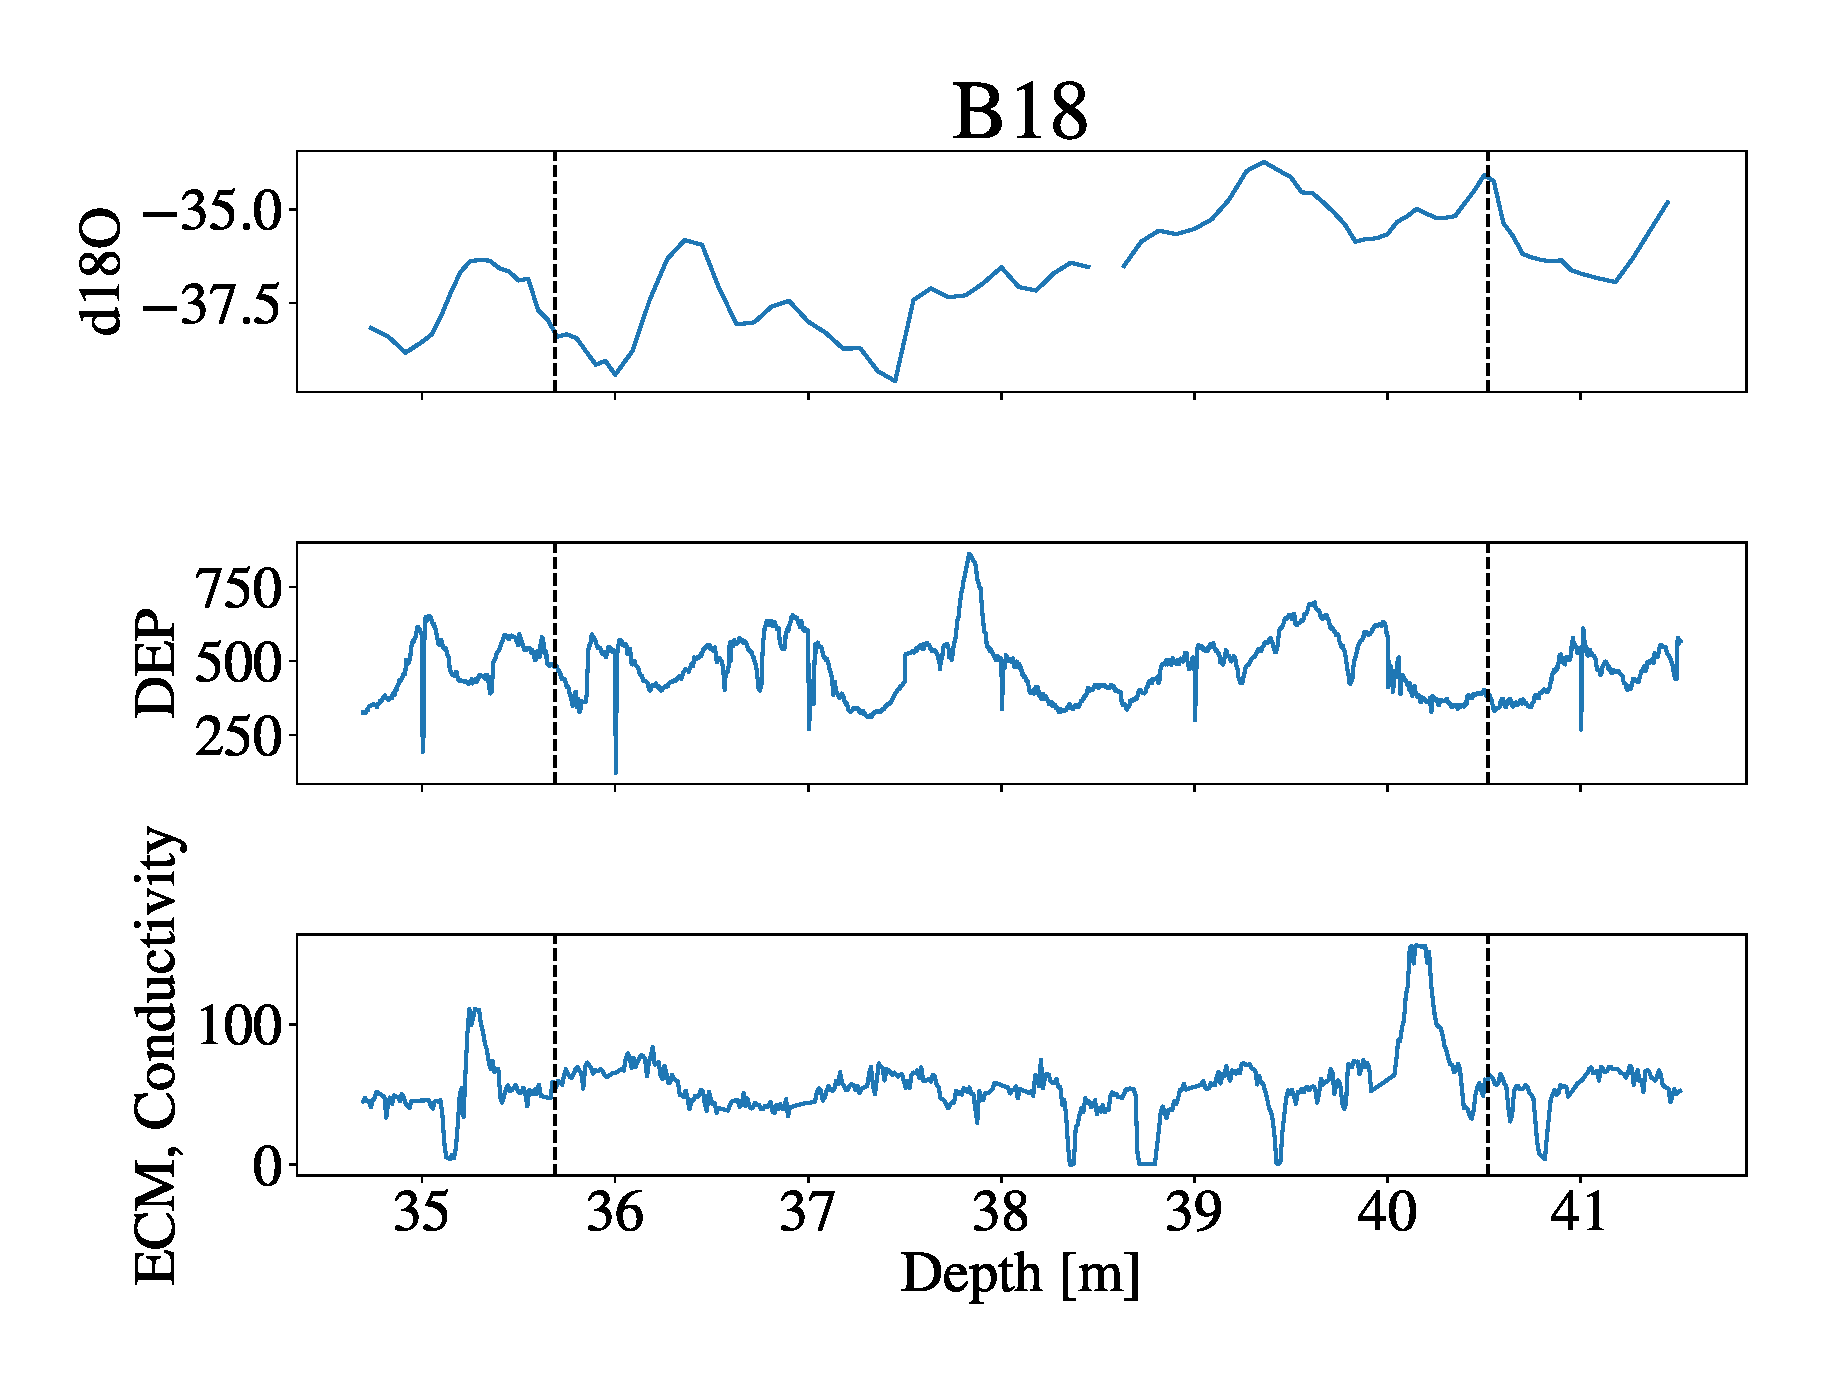
\includegraphics[width =0.3\linewidth]{Core_LT_B18.eps} & 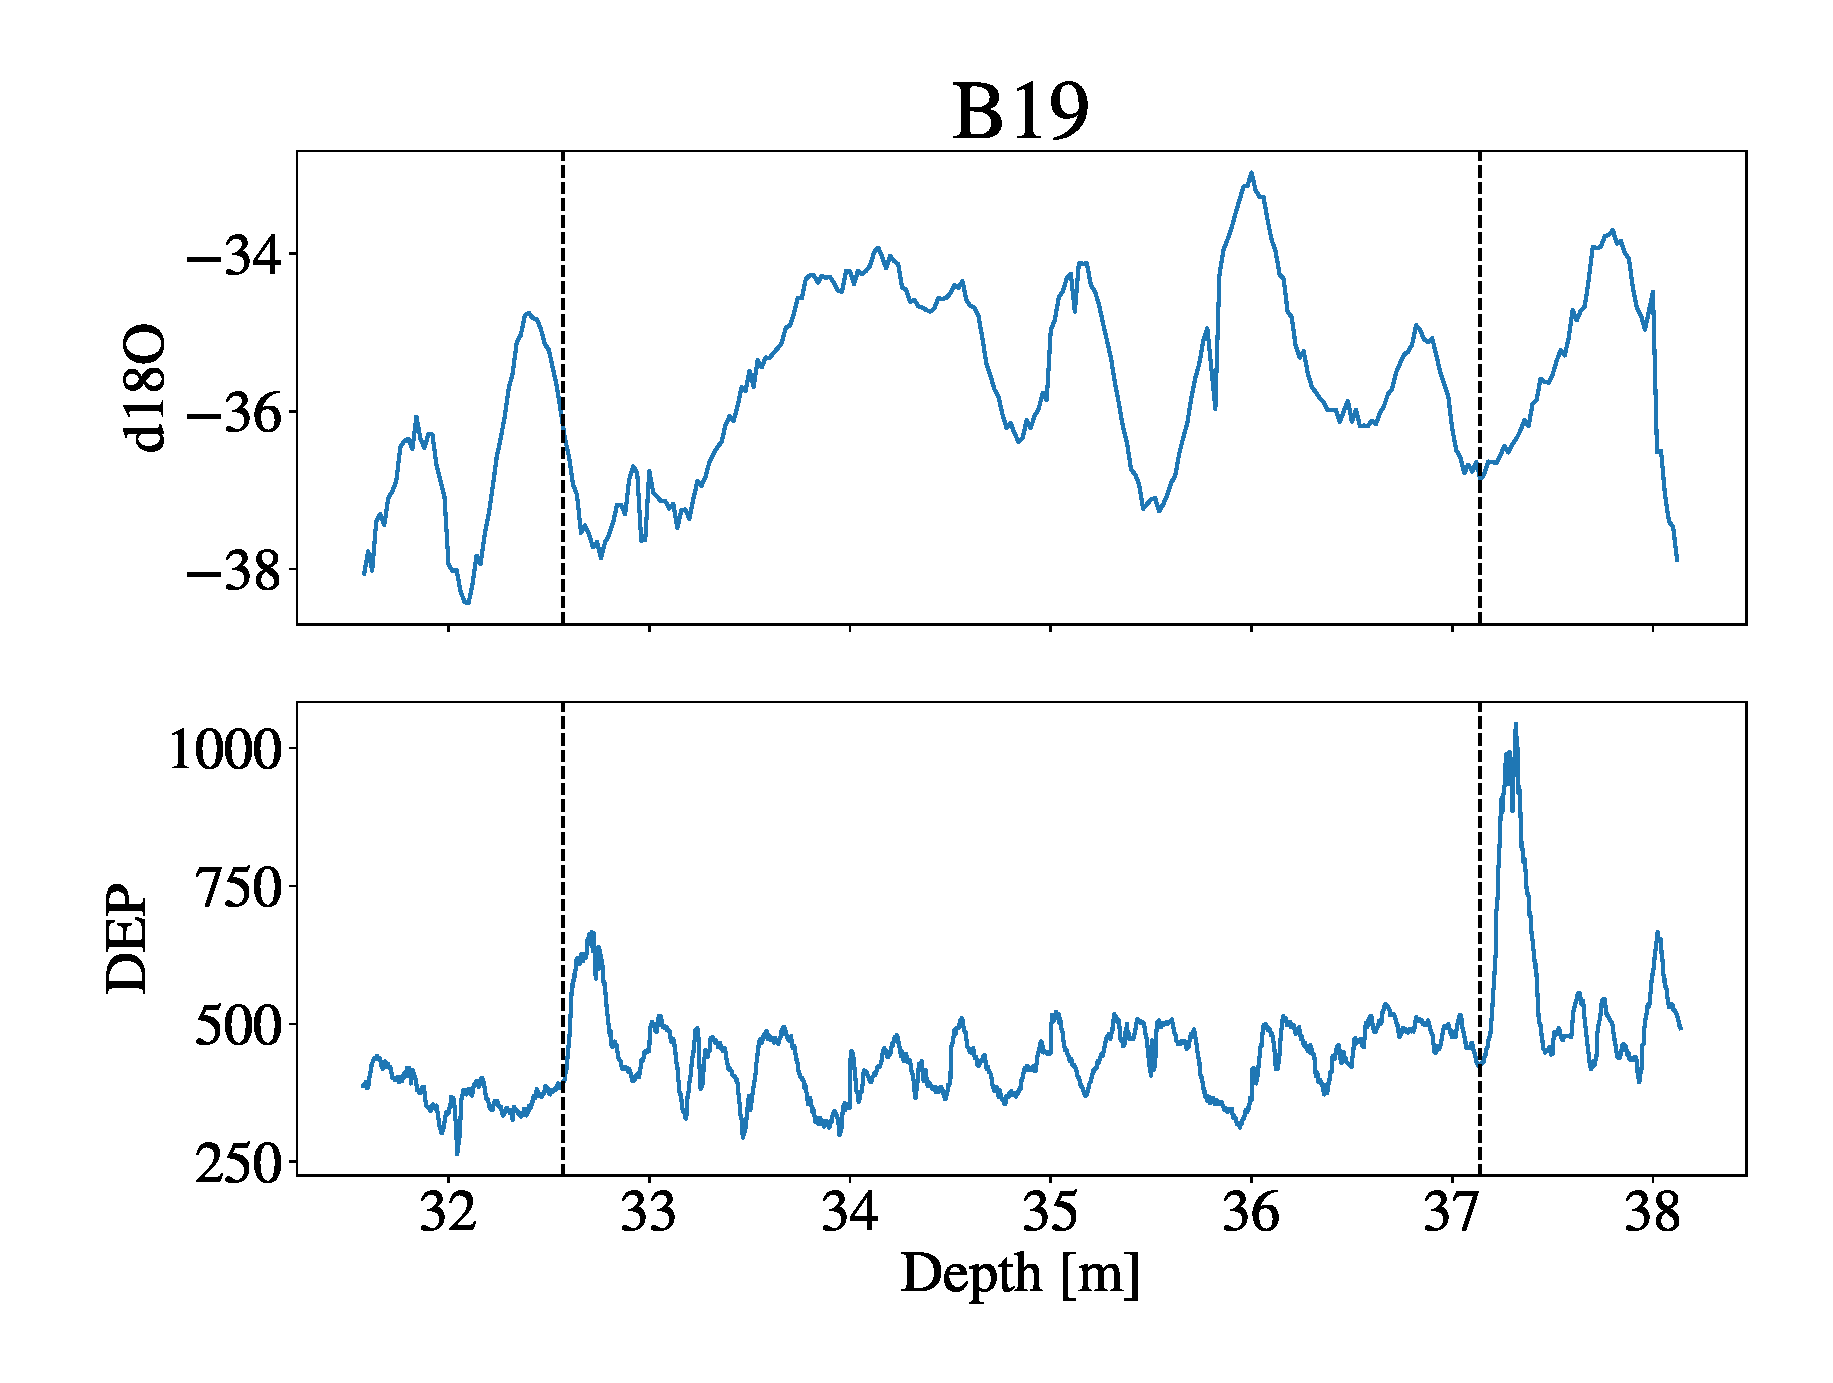
\includegraphics[width =0.3\linewidth]{Core_LT_B19.eps} \\
				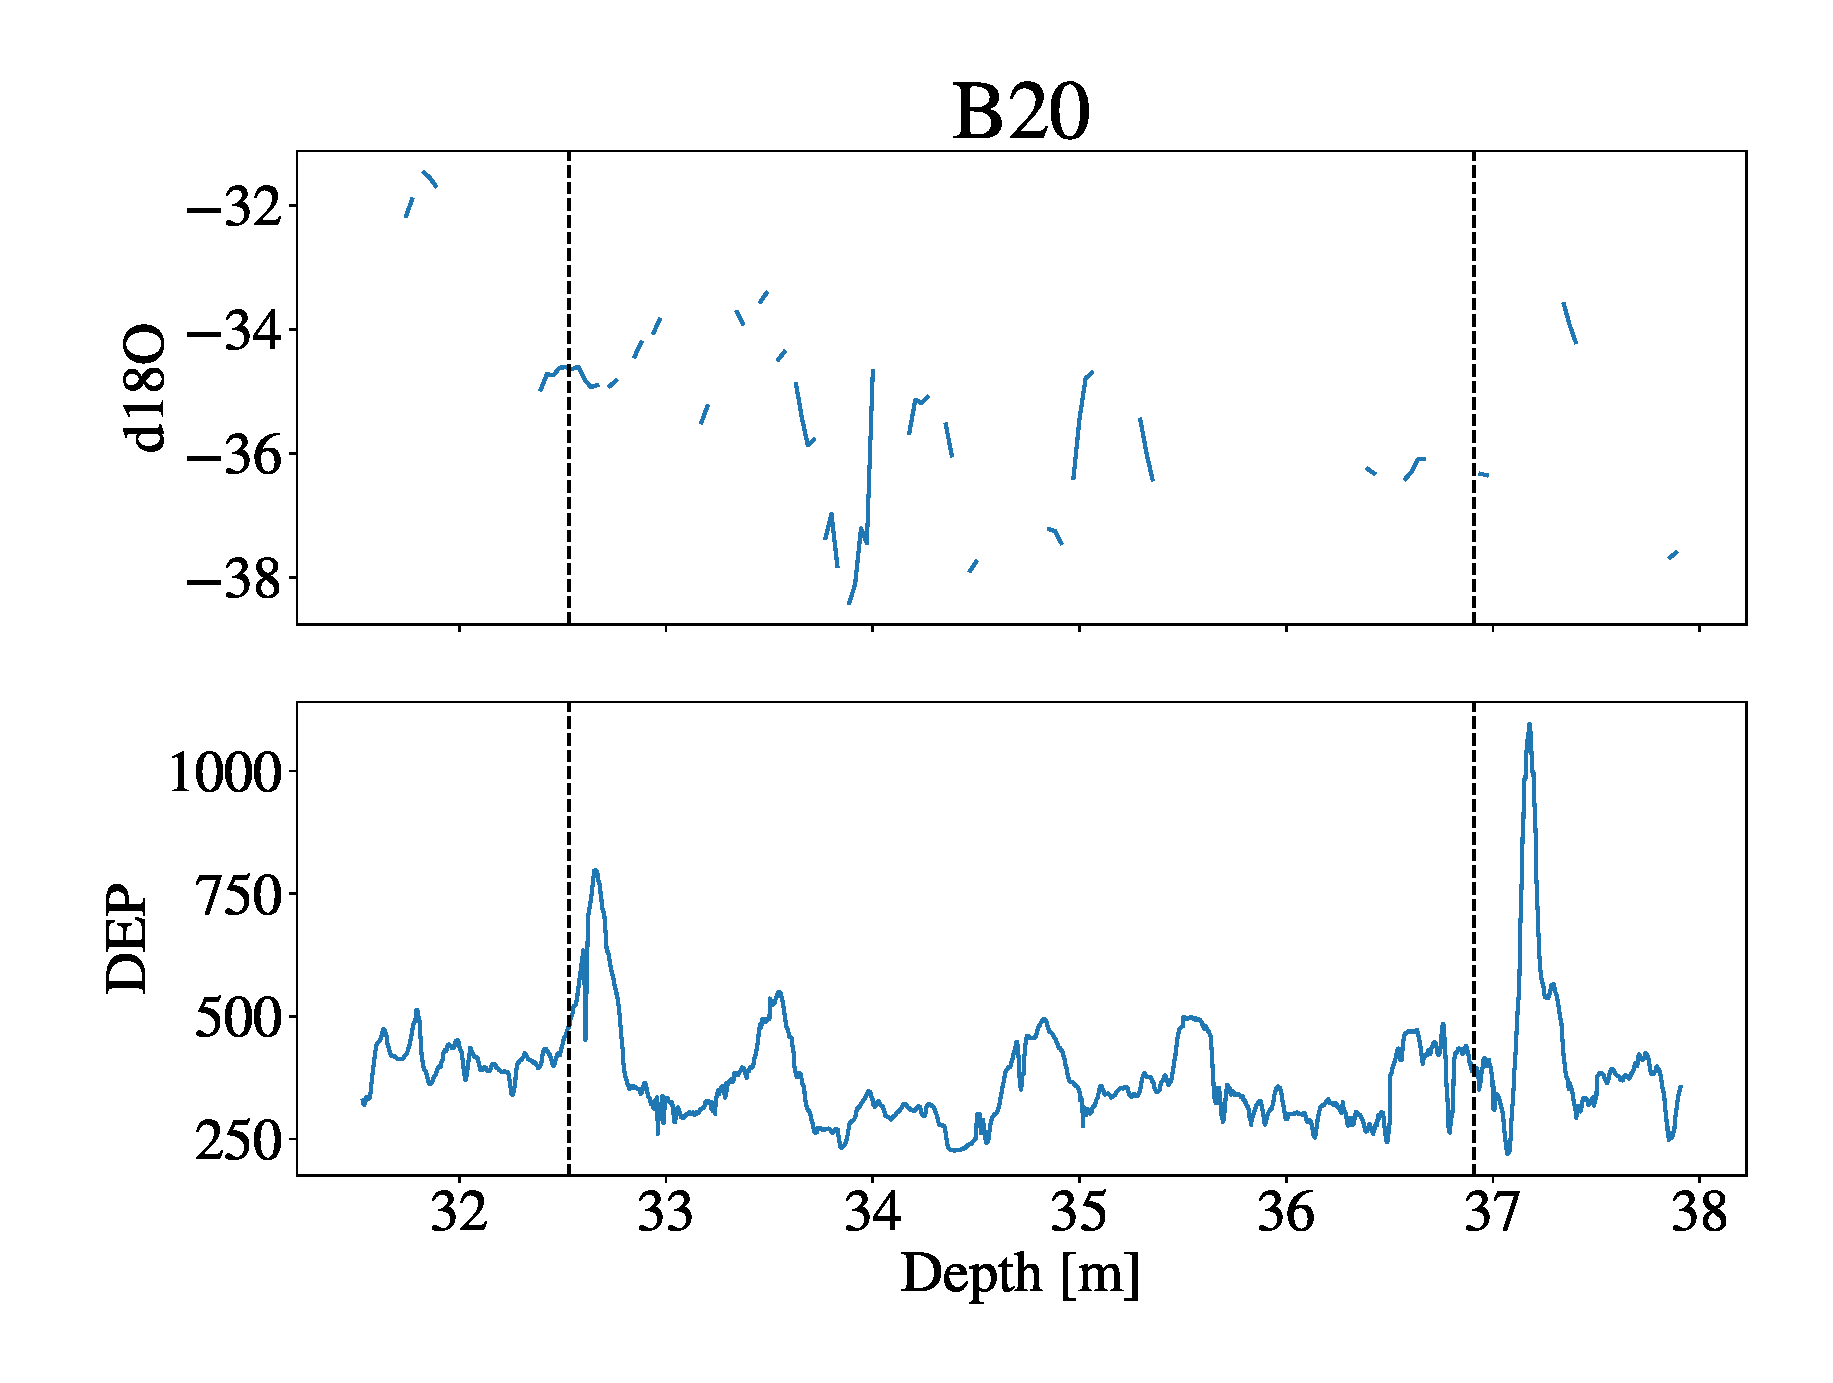
\includegraphics[width =0.3\linewidth]{Core_LT_B20.eps} & 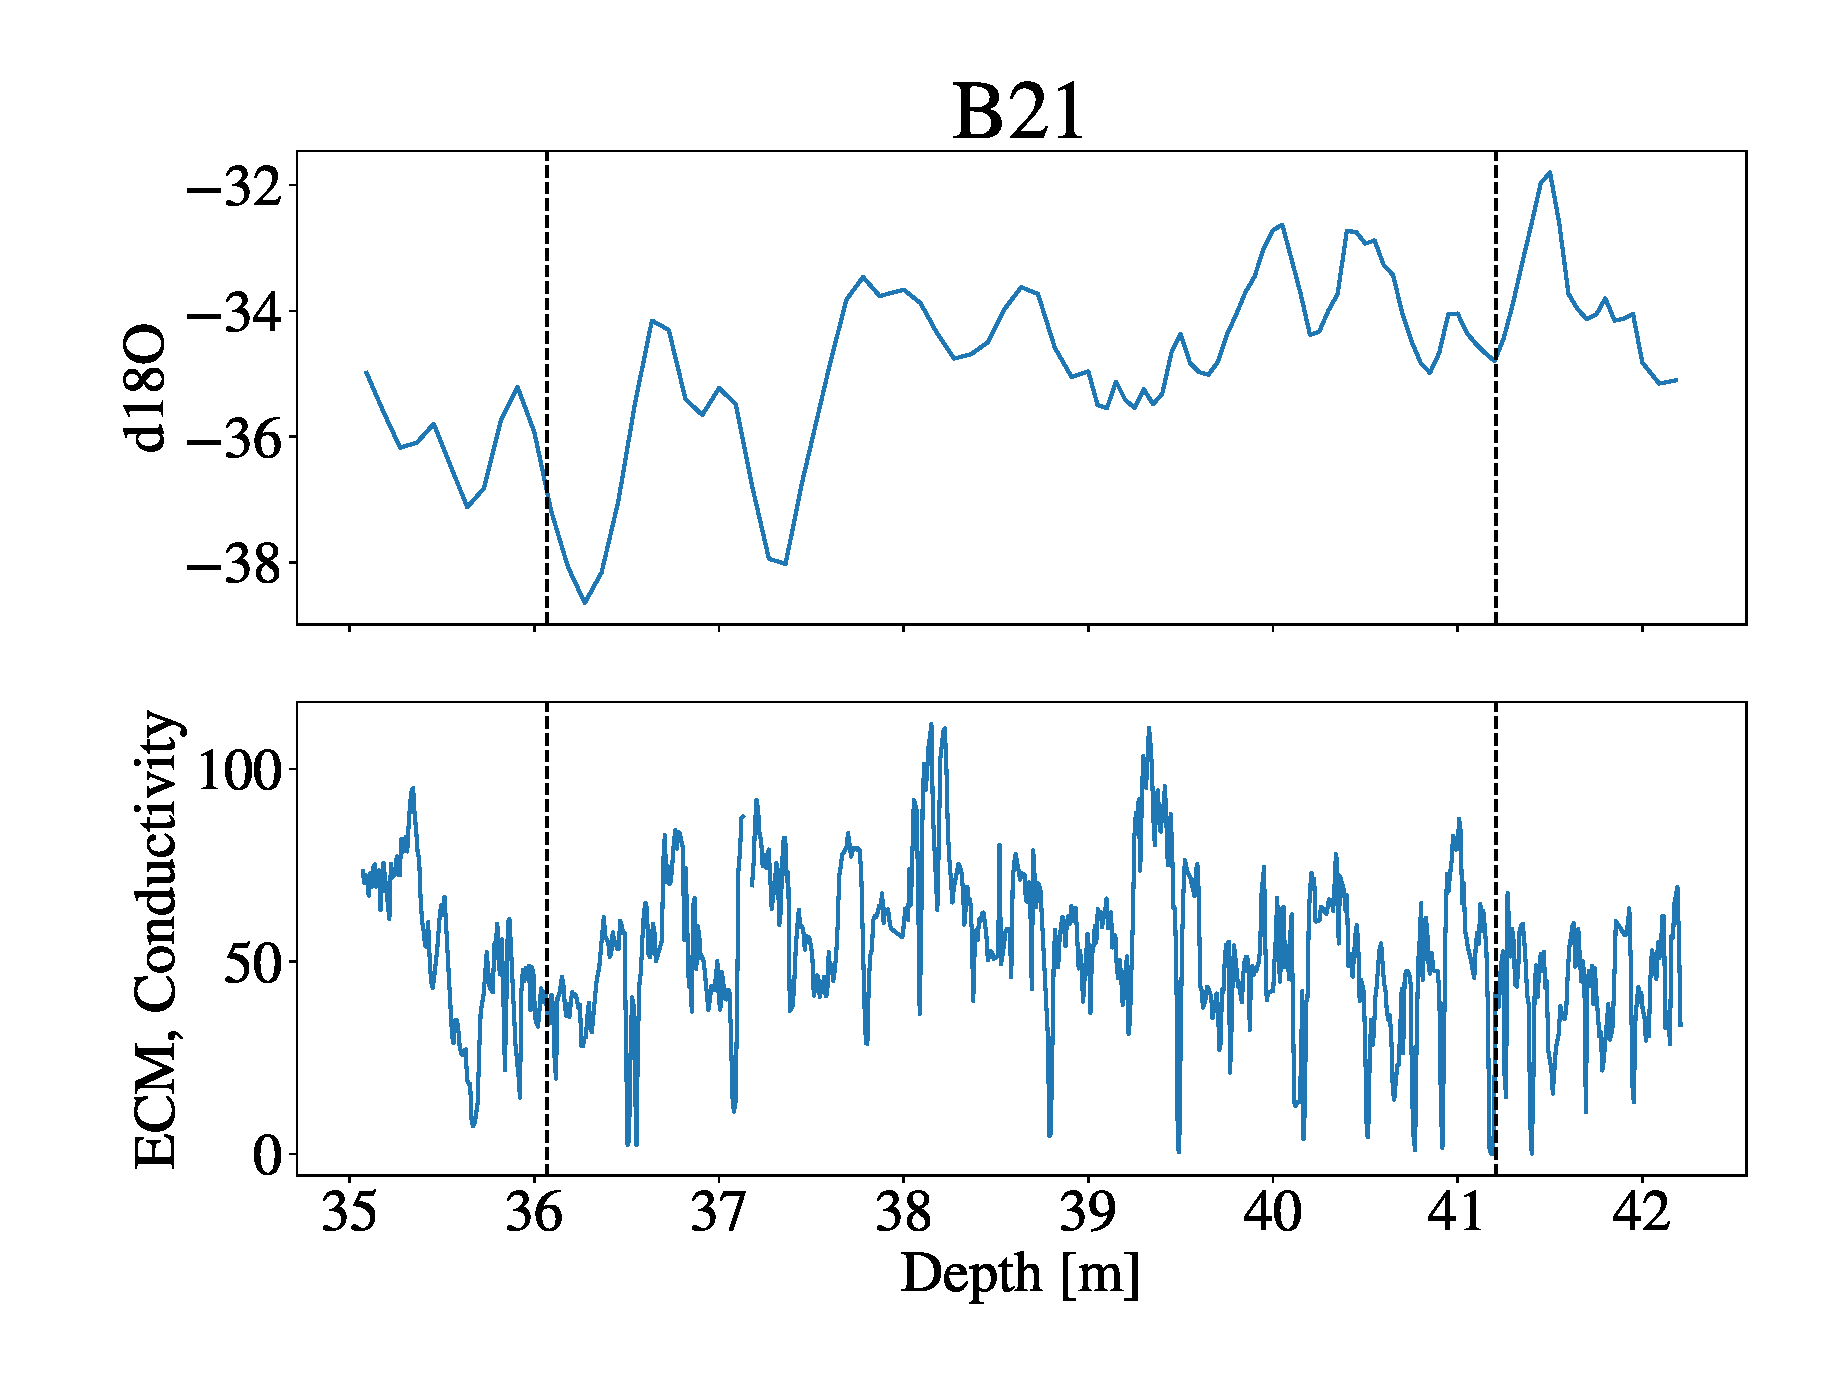
\includegraphics[width =0.3\linewidth]{Core_LT_B21.eps} & 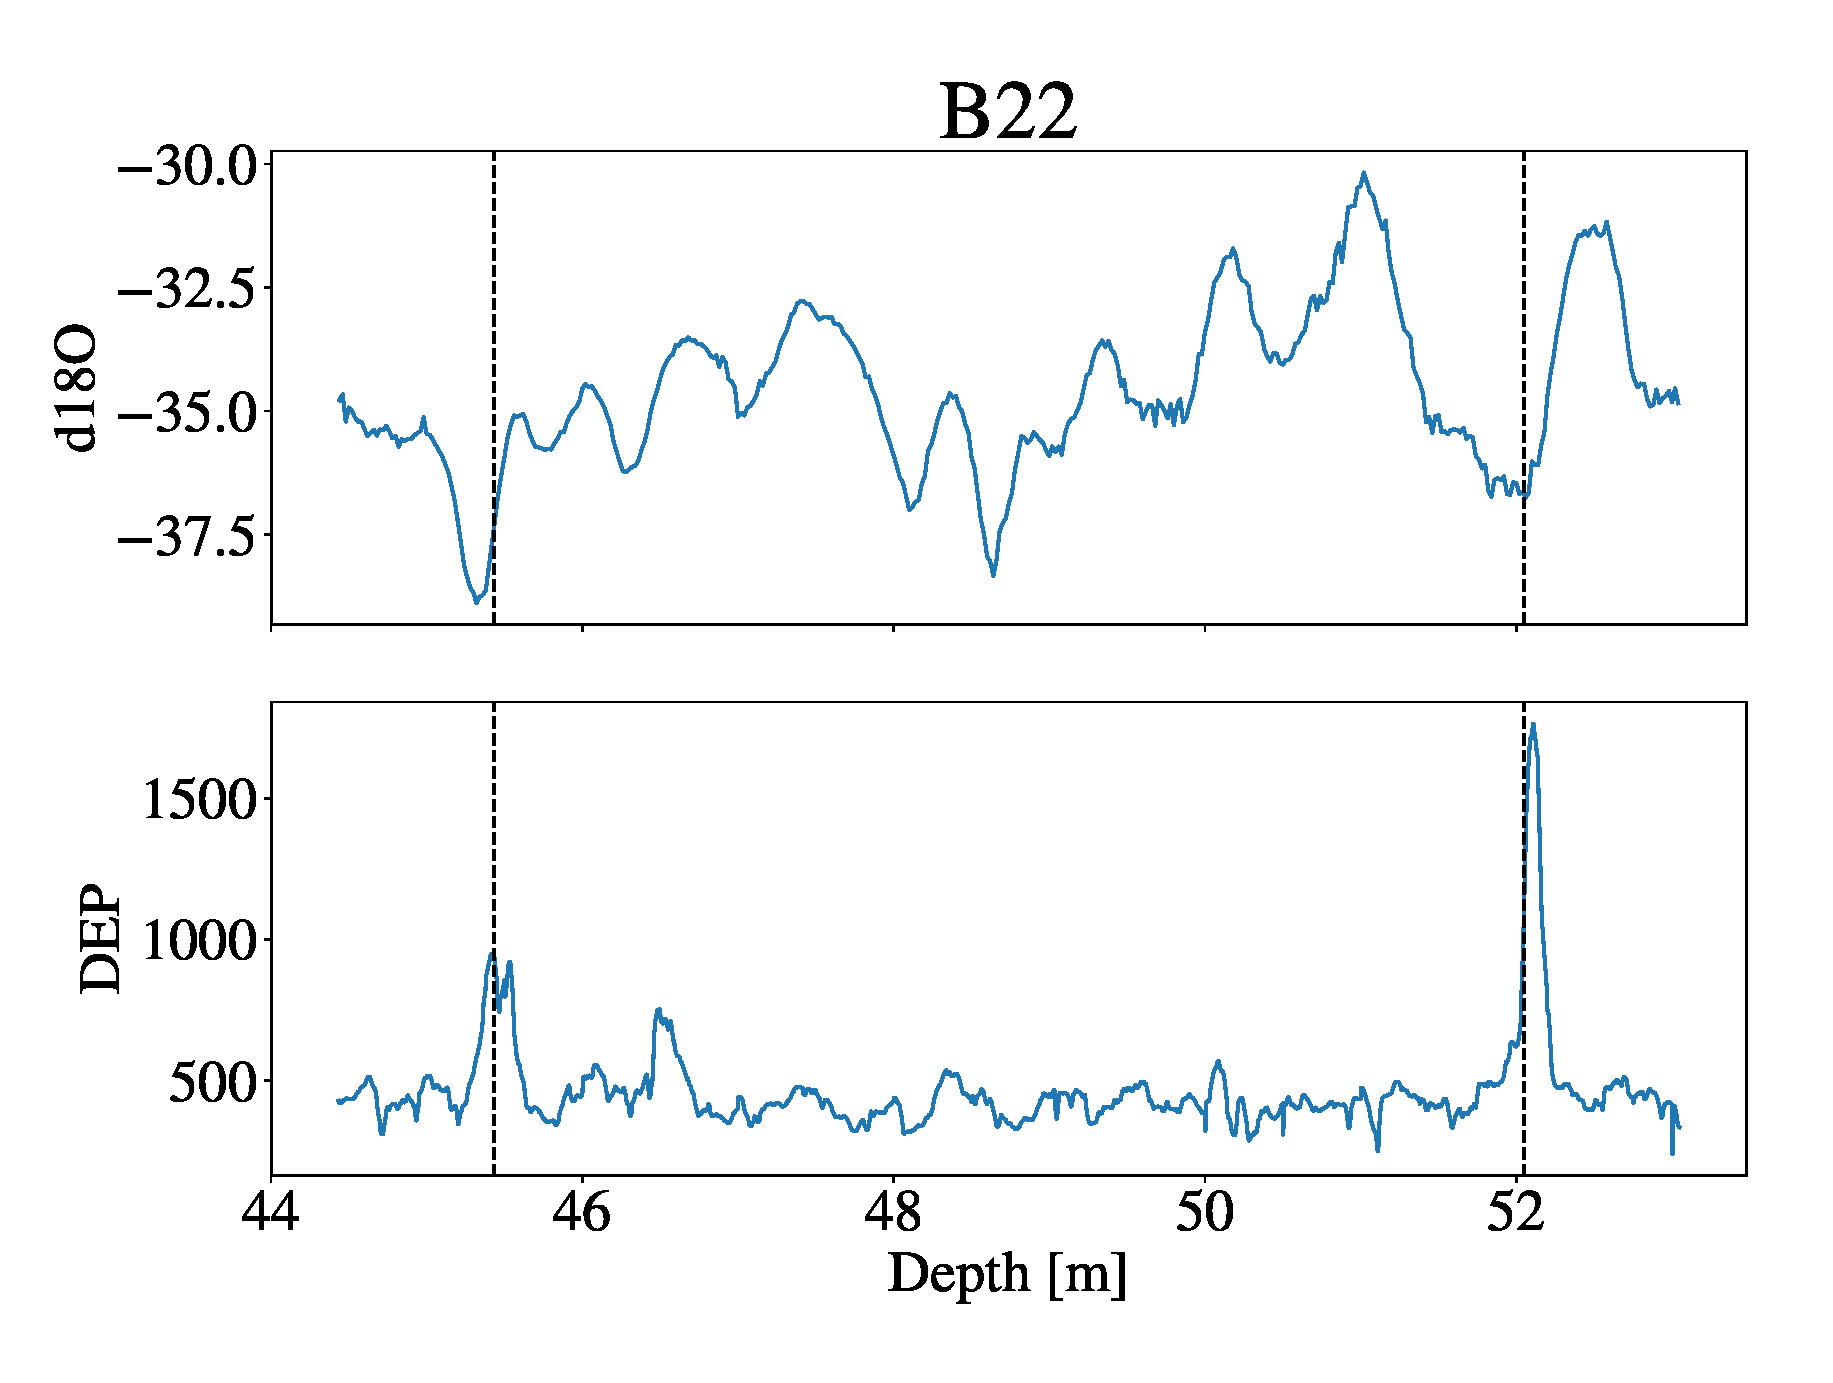
\includegraphics[width =0.3\linewidth]{Core_LT_B22.eps} \\	
				& & 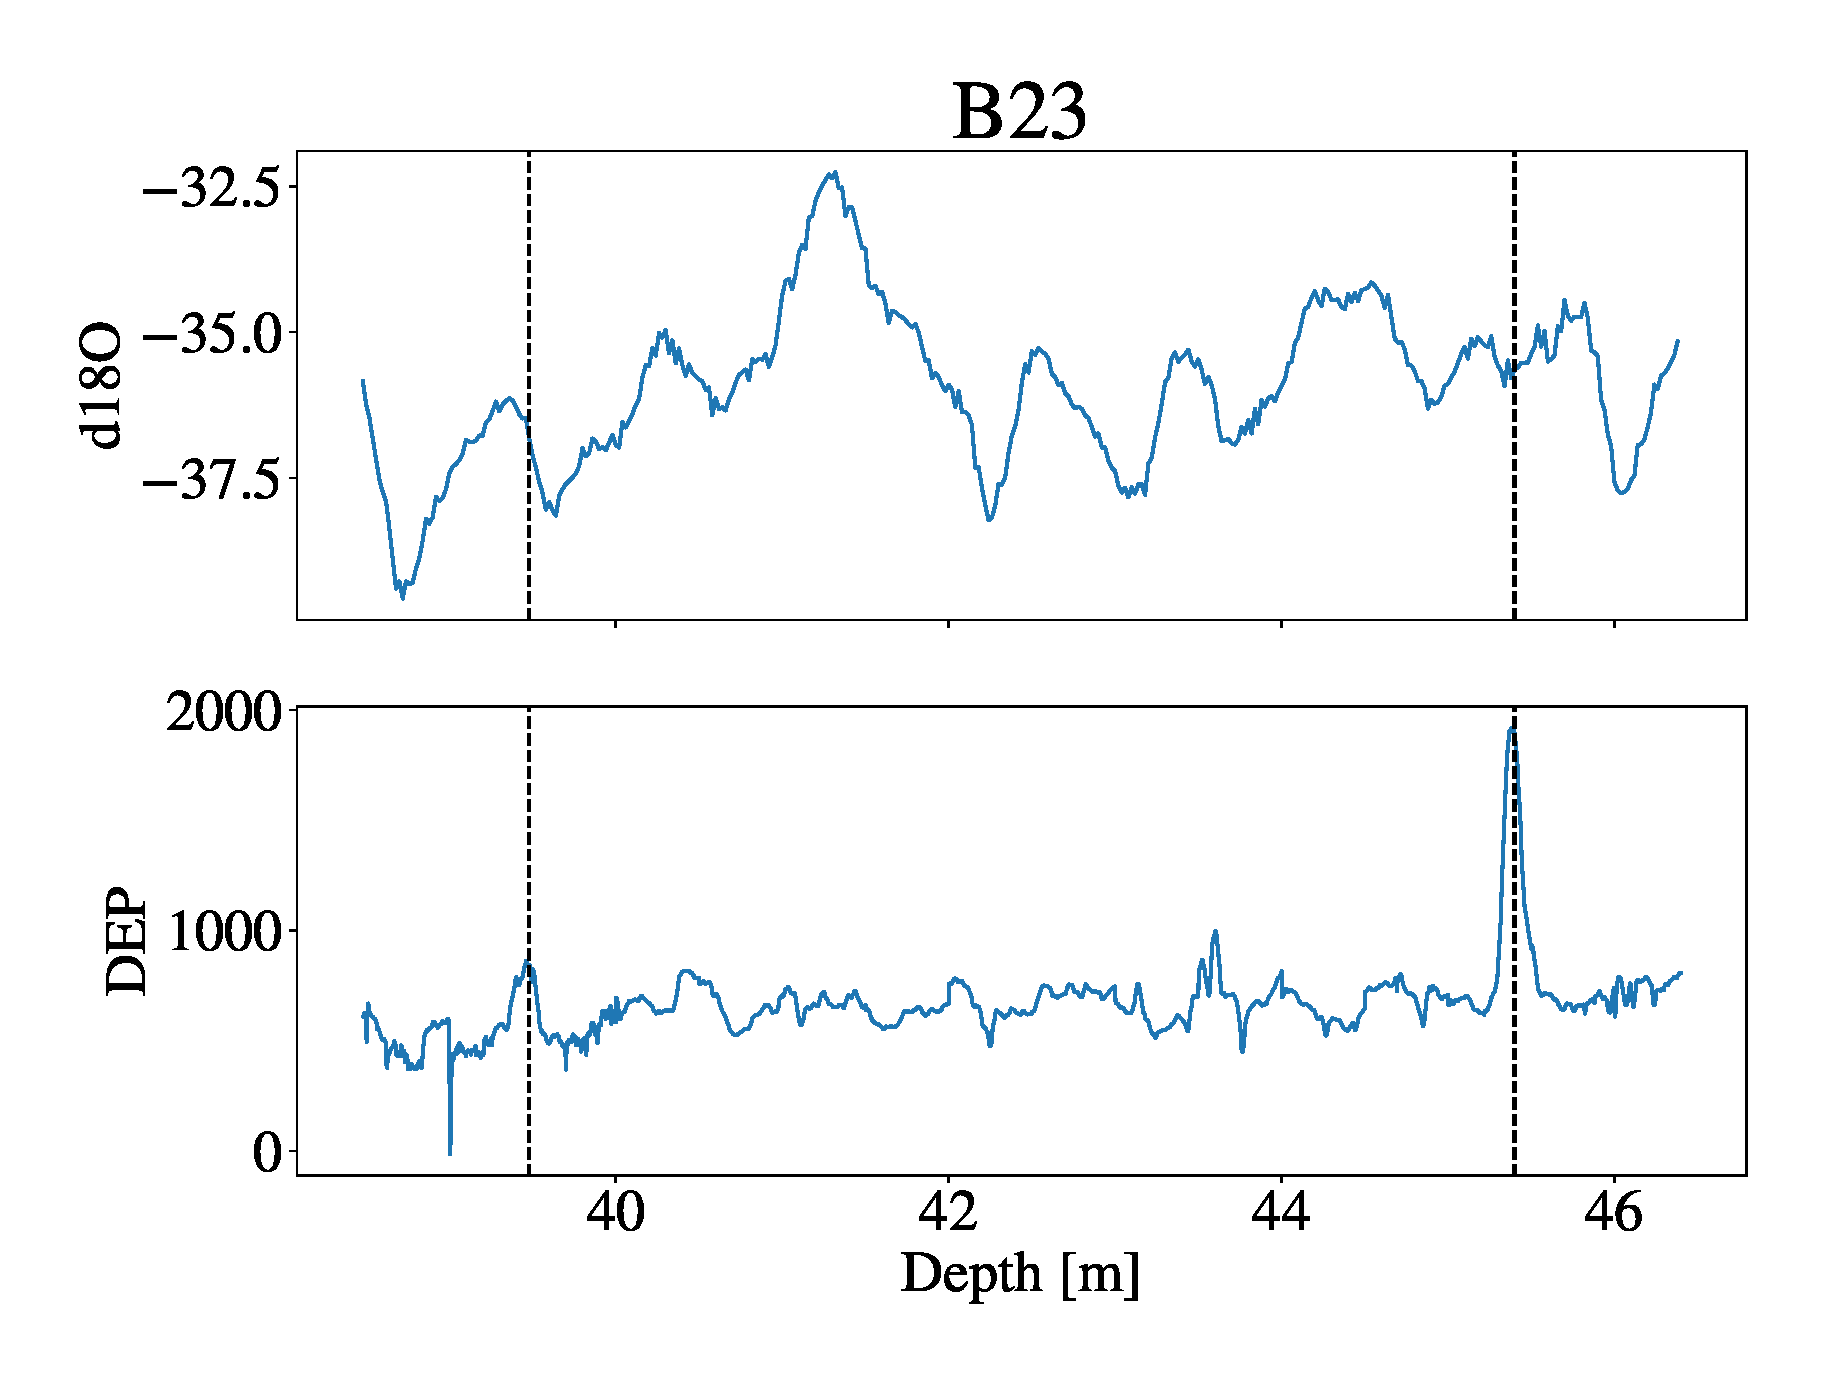
\includegraphics[width =0.3\linewidth]{Core_LT_B23.eps} \\
			\end{tabular}
		\end{table}
	\end{landscape}
\end{rotatepage}
\newpage

\begin{rotatepage}
	\begin{landscape}
		\begin{figure}[h]
			\centering
			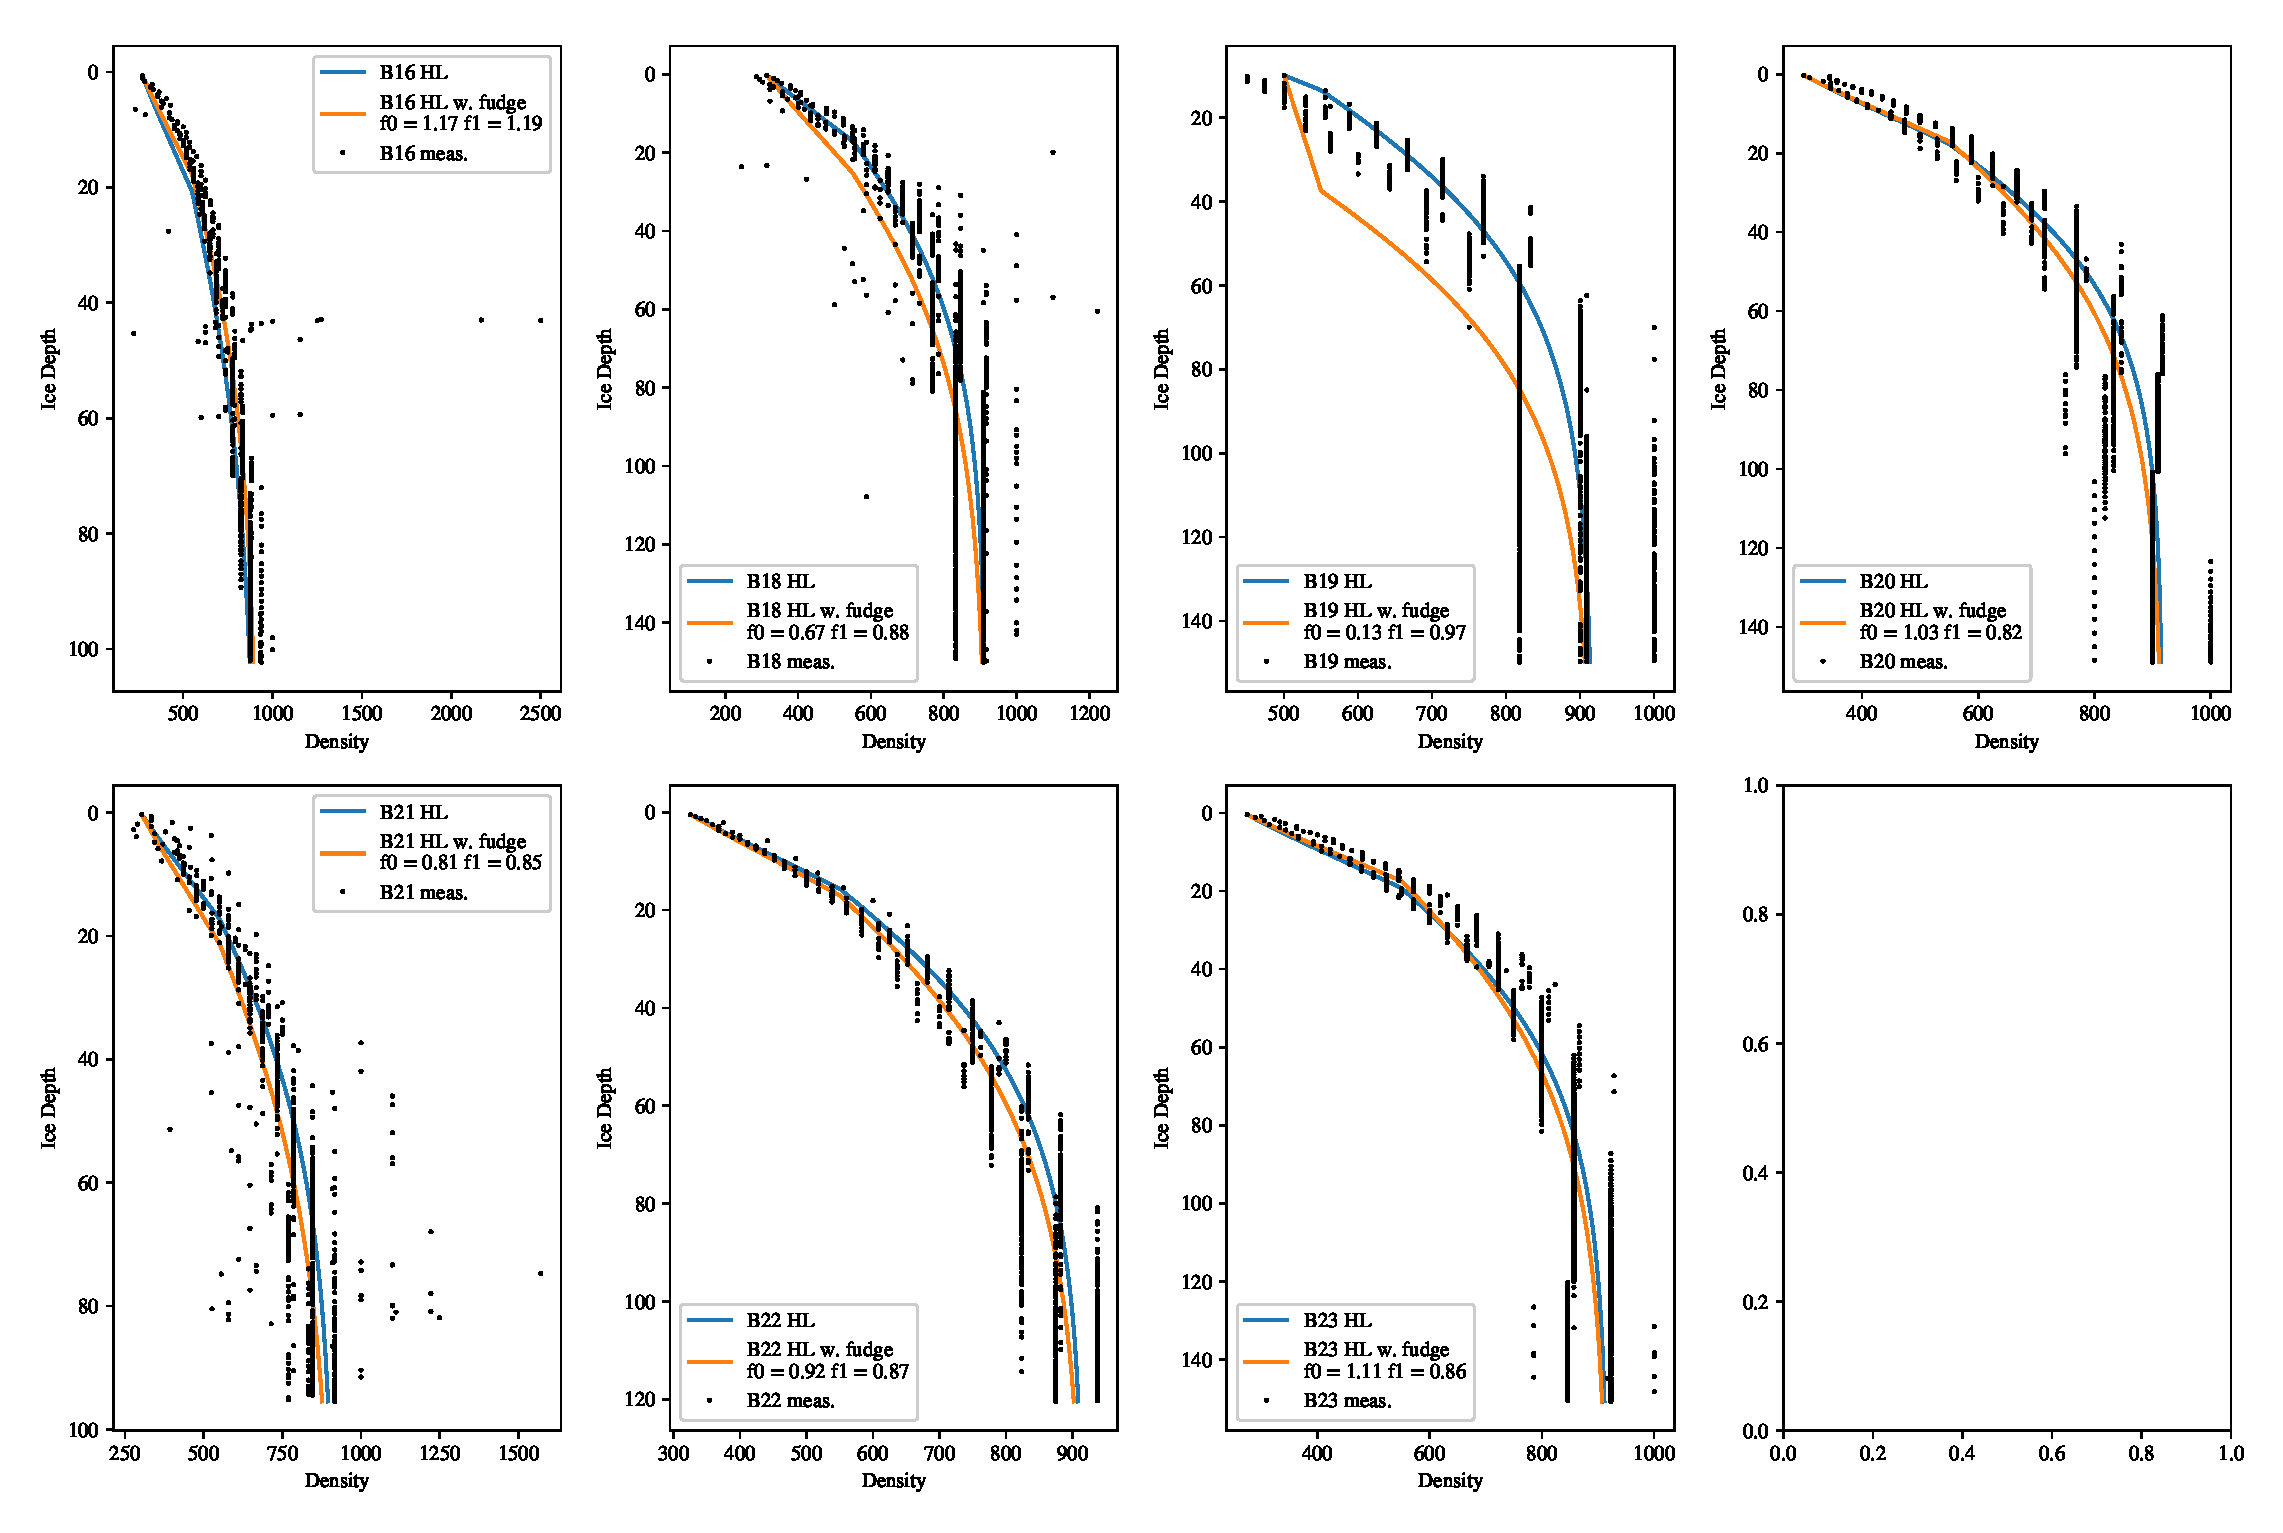
\includegraphics[width=1.5\textwidth]{fig_dens_B16B18B19B20B21B22B23.eps}
			\label{fig:dens}
			\caption{}
		\end{figure}
	\end{landscape}
\end{rotatepage}
\newpage
\begin{rotatepage}
	\begin{landscape}
		\begin{figure}[h]
			\centering
			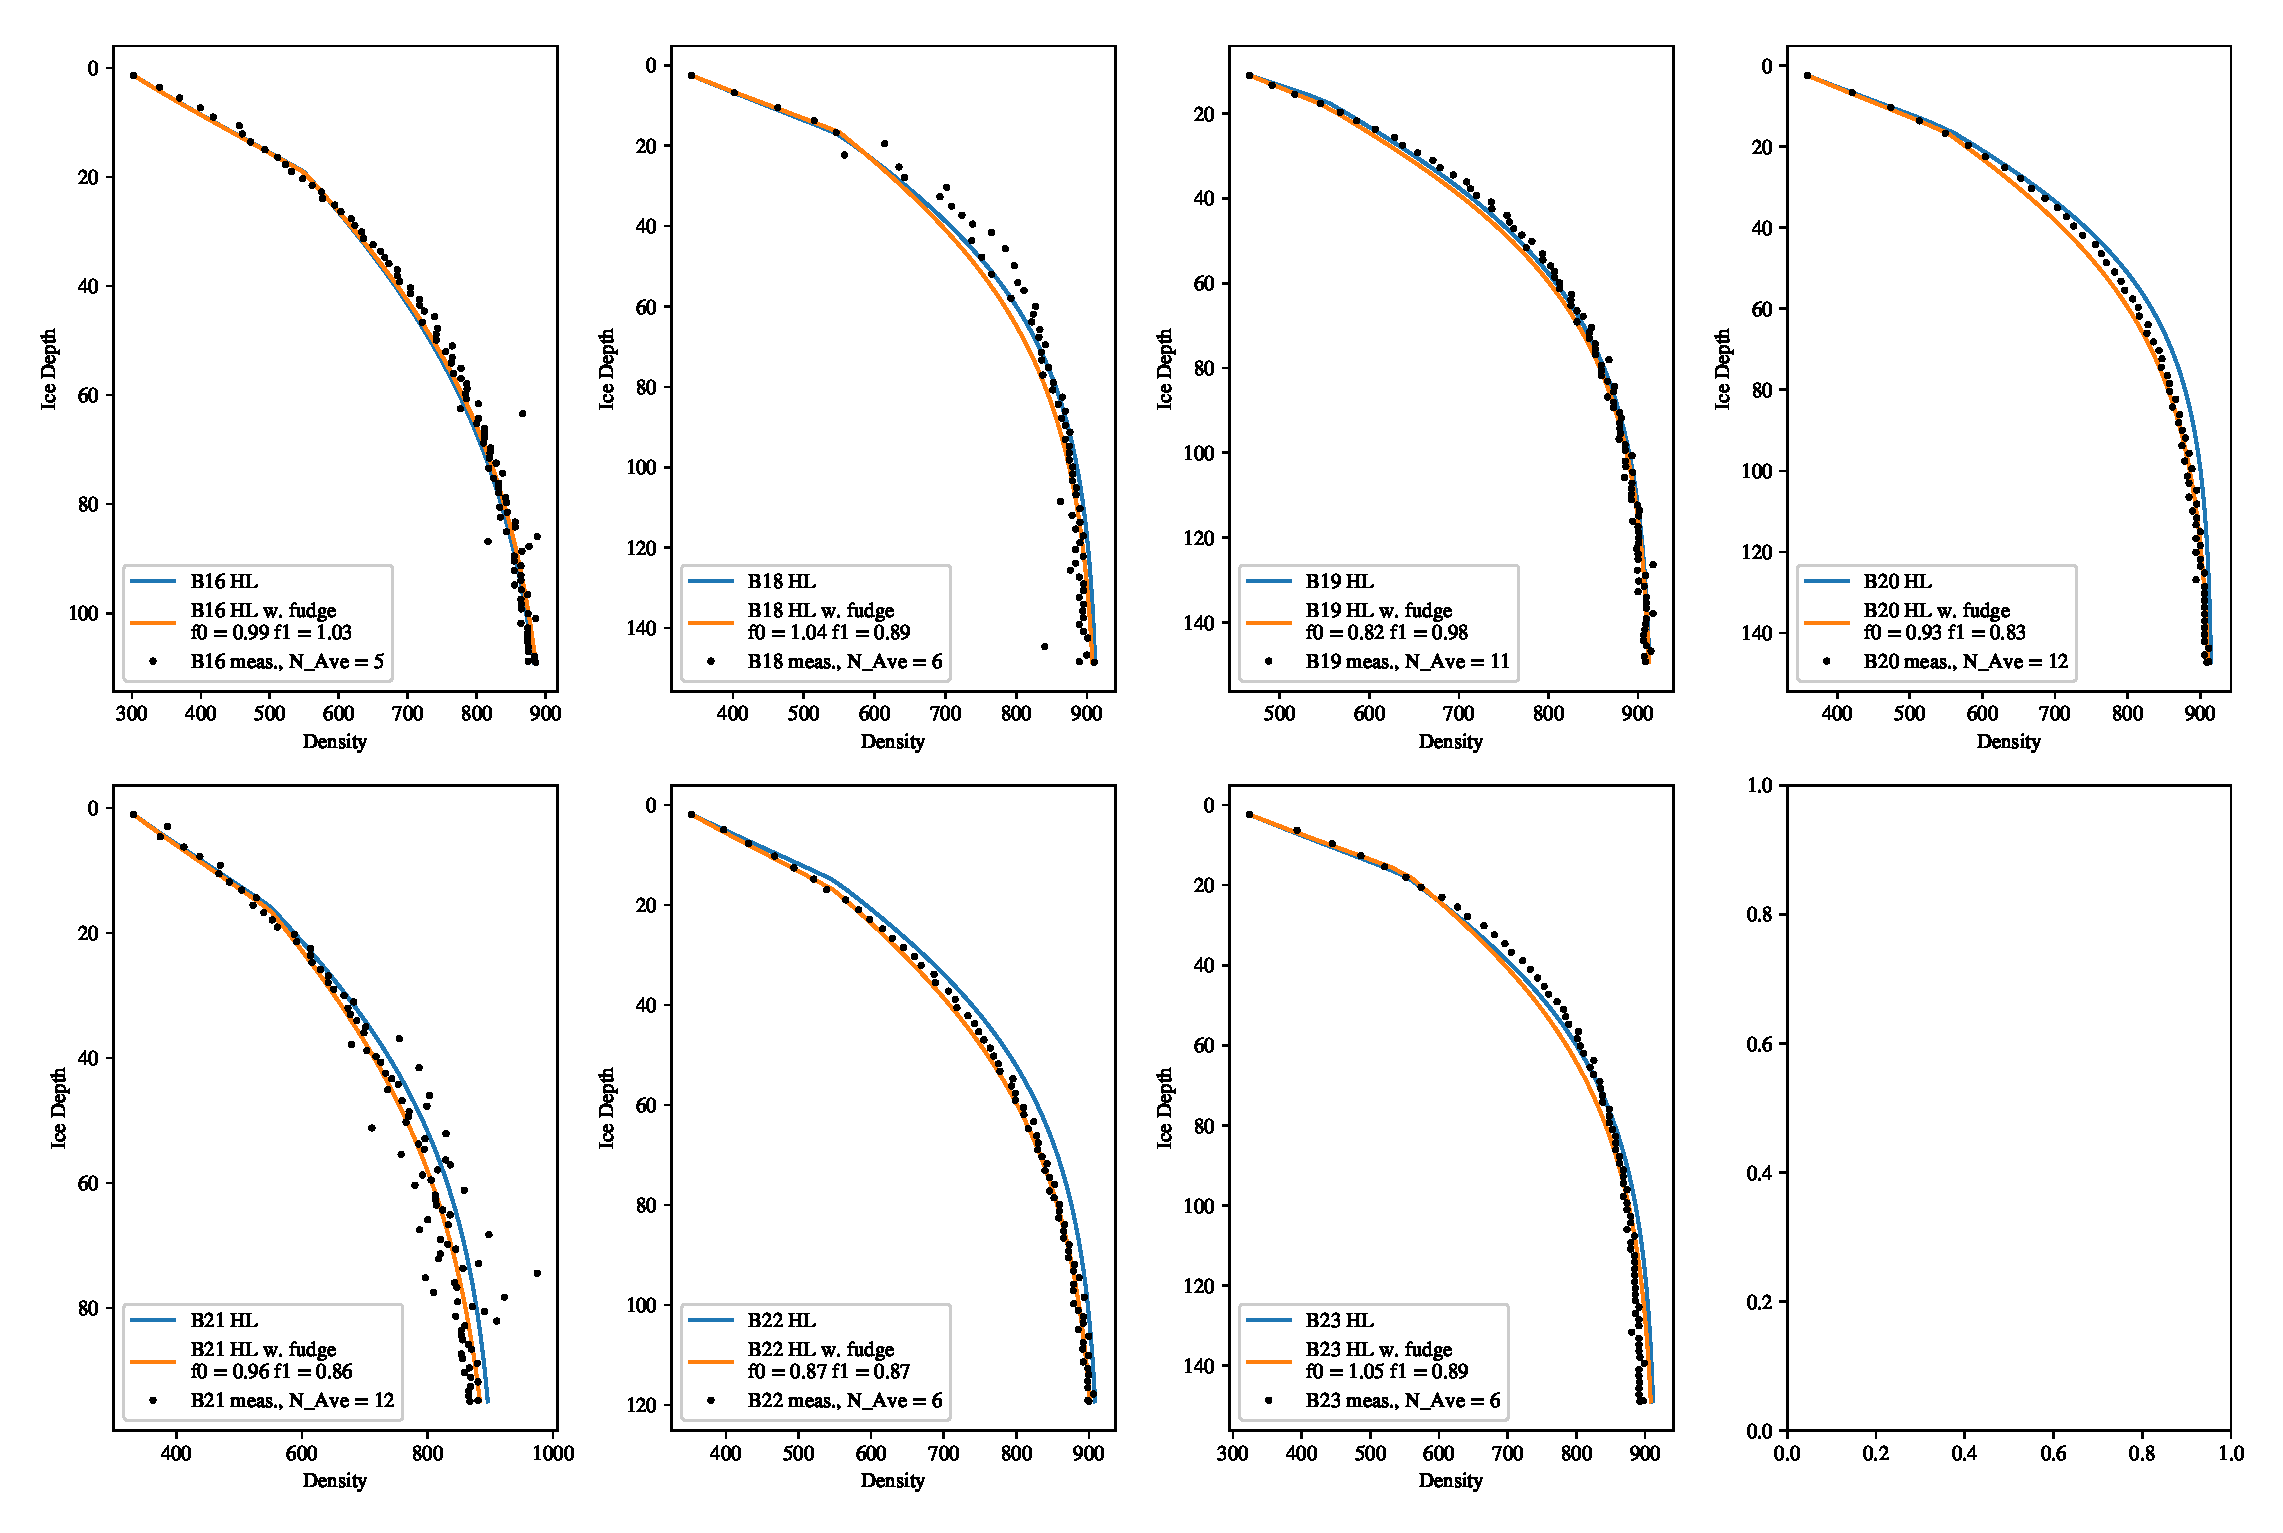
\includegraphics[width=1.5\textwidth]{fig_densAve_B16B18B19B20B21B22B23.eps}
			\label{fig:densAve}
			\caption{}
		\end{figure}
	\end{landscape}
\end{rotatepage}
\newpage 


\section[Appendix II]{Data: Alphabet Cores}
\label{App:Data_Alphabet}
\begin{figure}[h]
	\centering
	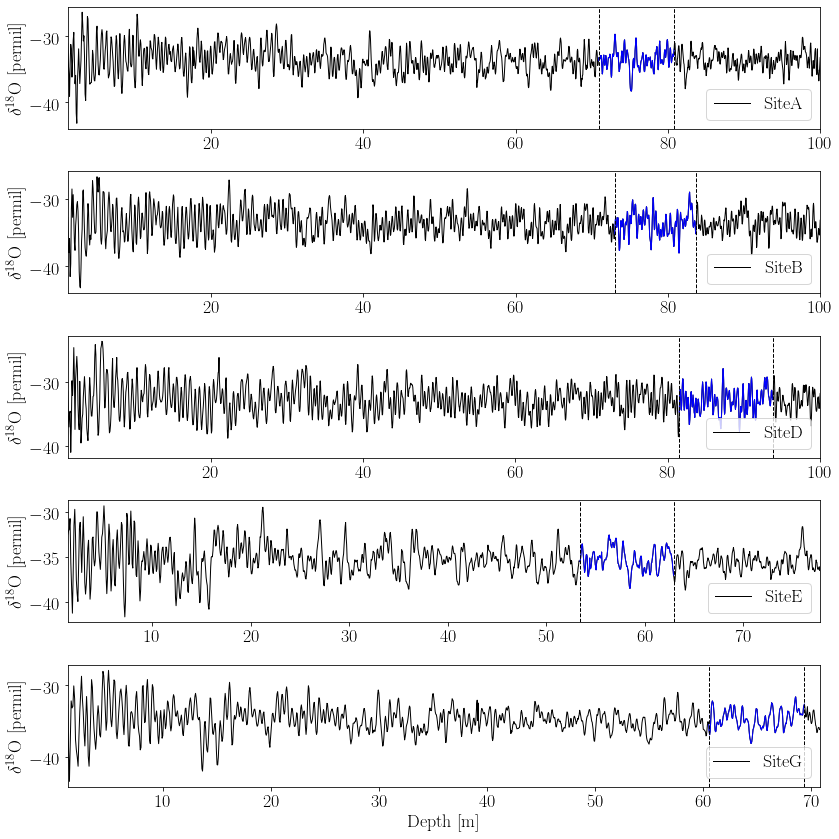
\includegraphics[width=0.9\textwidth]{AllAlphabetCores.png}
	\caption[]{}
	\label{fig:AllAlphabetCores}
\end{figure}

\begin{figure}[h]
	\centering
	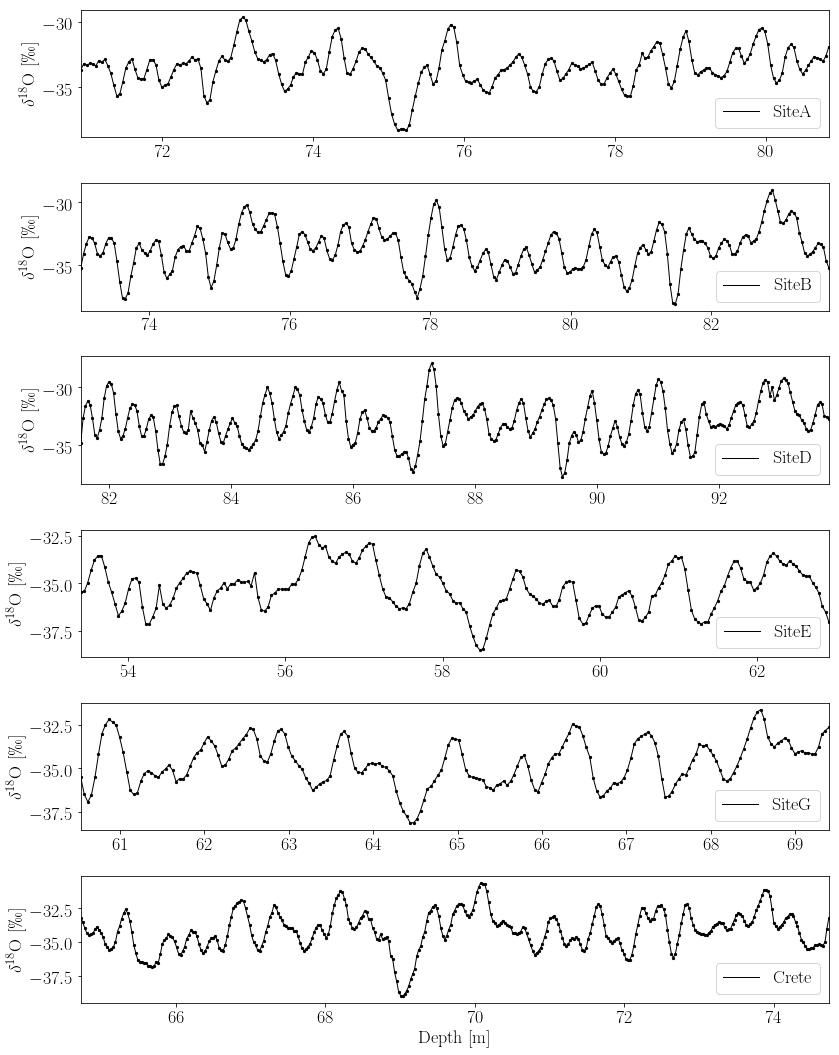
\includegraphics[width=\textwidth]{AllAlphabetCores_LT.png}
	\caption[]{}
	\label{fig:AllAlphabetCores_LT}
\end{figure}


\end{document}